\section{Edges}
%<-------------------------------------------------------------------------->
\subsection{\tkzcname{Edge}}
\begin{NewMacroBox}{Edge}{\oarg{local options}\varp{vertex A}\varp{vertex B}}
\begin{tabular}{llc}
\toprule
Options              & Default     & Definition       \\
\midrule
\TOline{color}       {\textbackslash EdgeColor}     {color of the edge}
\TOline{lw}          {\textbackslash EdgeLineWidth} {line width of the edge}
\TOline{double}      {\{\}}   {color of the border of a double edge}
\TOline{dd}          {\textbackslash EdgeDoubleDistance}{line width of the border}
\TOline{label}       {\{\}}   {label of the edge}
\TOline{labeltext}   {\textbackslash LabelTextColor}{color of the text of the label}
\TOline{labelcolor}  {\textbackslash LabelFillColor}{color of the background of the label}
\TOline{labelstyle}  {\{\}}   {\TIKZ\ options of the label}
\TOline{style}       {pos=.5} {\TIKZ\ options of the edge}
\TOline{local}       {false}  {the style \tkzname{EdgeStyle} is not used}
\midrule
\TOline{->}          {}       {arrow from A to B}
\TOline{<-}          {}       {arrow from B to A}
\TOline{<->}         {}       {arrows at both ends}
\TOline{-}           {}       {no arrow}
\TOline{arrow}       {\{\}}   {any \TIKZ\ arrow specification}
\bottomrule
\end{tabular}

\medskip
\emph{\tkzcname{Edge} draws an edge between two vertices. The edge uses the
style \tkzname{EdgeStyle} (defined by \tkzcname{GraphInit}) and its label the
style \tkzname{LabelStyle}. The keys \tkzname{->}, \tkzname{<-} and
\tkzname{<->} use the tip given by \tkzcname{tkzSetUpGraph}\tkzname{[arrow
tip=\dots]} (\tkzname{stealth'} by default).}
\end{NewMacroBox}

\subsubsection{Straight edges and arcs}
An edge is a segment or an arc; it can have a label. The style
\tkzname{EdgeStyle} can be redefined for all the following edges.

\begin{tkzexample}[latex=8cm,small]
\begin{tikzpicture}
  \SetGraphUnit{4}
  \Vertex{a}
  \EA(a){b}
  \SO[unit=2](a){c}
  \EA(c){d}
  {\SetGraphUnit{2}
  \SO(c){e}}
  \EA(e){f}
  \Edge(a)(b)
  \tikzset{EdgeStyle/.style = {bend left}}
  \Edge(c)(d)
  \tikzset{EdgeStyle/.style = {bend right=60}}
  \Edge[->](e)(f)
\end{tikzpicture}
\end{tkzexample}

\subsubsection{The option \tkzname{style}}
\begin{tkzexample}[latex=8cm,small]
\begin{tikzpicture}
  \SetGraphUnit{4}
  \Vertex{e}
  \EA(e){f}
  \Edge(f)(e)
  \Edge[style={bend left}](f)(e)
  \Edge[style={bend right}](f)(e)
\end{tikzpicture}
\end{tkzexample}

\subsubsection{Arrows}
\begin{tkzexample}[latex=8cm,small]
\begin{tikzpicture}
  \SetGraphUnit{2}
  \Vertices{line}{A,B,C,D}
  \Edge[->](A)(B)
  \Edge[<->,color=red](B)(C)
  \Edge[<-,style={bend left}](C)(D)
  \Edge[arrow={-to},style={bend right}](C)(D)
\end{tikzpicture}
\end{tkzexample}

\subsubsection{Double edges}
\tkzname{double} gives the color of the border, \tkzname{lw} the width of
the inside and \tkzname{dd} the width of the border.

\begin{tkzexample}[latex=8cm,small]
\begin{tikzpicture}
  \SetGraphUnit{4}
  \Vertex{A} \EA(A){B}
  \Edge[double=black,color=orange,lw=2pt](A)(B)
\end{tikzpicture}
\end{tkzexample}

\subsubsection{Labels}
\begin{tkzexample}[latex=8cm,small]
\begin{tikzpicture}
  \SetGraphUnit{4}
  \Vertex{A} \EA(A){B} \NO(B){C}
  \Edge[label=$5$](A)(B)
  \Edge[label=$7$,labelcolor=yellow,labeltext=red](B)(C)
  \Edge[label=$2$,labelstyle={draw,sloped}](C)(A)
\end{tikzpicture}
\end{tkzexample}

\newpage
\subsection{\tkzcname{Edges}}
\begin{NewMacroBox}{Edges}{\oarg{local options}\varp{vertex A,vertex B,\dots}}
\emph{\tkzcname{Edges} draws a chain of edges A--B, B--C\dots. The options
are those of \tkzcname{Edge}; they apply to every edge.}
\end{NewMacroBox}

\begin{tkzexample}[latex=7cm,small]
\begin{tikzpicture}
  \GraphInit[vstyle=Art]
  \Vertices[unit=2]{circle}{a0,a1,a2,a3,a4,a5,a6,a7}
  \Edges(a0,a3,a6,a1,a4,a7,a2,a5,a0)
\end{tikzpicture}
\end{tkzexample}

\begin{tkzexample}[latex=7cm,small]
\begin{tikzpicture}
  \Vertices[unit=2,rotation=90]{circle}{A,B,C,D,E}
  \Edges[->,color=blue](A,B,C,D,E,A)
\end{tikzpicture}
\end{tkzexample}

\subsection{A loop: \tkzcname{Loop}}
\begin{NewMacroBox}{Loop}{\oarg{local options}\varp{vertex}}
\begin{tabular}{llc}
\toprule
Options              & Default     & Definition       \\
\midrule
\TOline{dir}         {WE}          {direction: WE, EA, NO, SO, NOWE, NOEA, SOWE, SOEA}
\TOline{dist}        {4cm}         {size of the loop}
\TOline{color}       {black}       {color of the loop}
\TOline{label}       {\{\}}        {label}
\TOline{labelstyle}  {\{\}}        {\TIKZ\ options of the label}
\TOline{style}       {pre,thick}   {\TIKZ\ options of the loop}
\bottomrule
\end{tabular}

\medskip
\emph{The direction is not case sensitive. \tkzcname{grLoop} is another name
of this macro, always defined.}
\end{NewMacroBox}

\begin{tkzexample}[vbox,small]
\begin{tikzpicture}
  \useasboundingbox (-2,-2) rectangle (8,2);
  \SetVertexSimple
  \SetGraphUnit{5}
  \Vertex{A}
  \EA(A){B}
  \Edge[->](A)(B)
  \Loop[dist=3cm,dir=EA,style={thick,->}](B)
  \Loop[dist=5cm,dir=WE,style={thick,->},label=$0.5$,labelstyle=left](A)
\end{tikzpicture}
\end{tkzexample}

\newpage
\subsection{Default values for the edges: \tkzcname{SetUpEdge}}
\begin{NewMacroBox}{SetUpEdge}{\oarg{local options}}
\begin{tabular}{llc}
\toprule
Options         & Default  & Definition                       \\
\midrule
\TOline{color}      {\textbackslash EdgeColor}     {color of the edges}
\TOline{lw}         {\textbackslash EdgeLineWidth} {line width}
\TOline{label}      {\{\}}                          {label}
\TOline{labeltext}  {\textbackslash LabelTextColor}{color of the text of the labels}
\TOline{labelcolor} {\textbackslash LabelFillColor}{background of the labels}
\TOline{labelstyle} {\{\}}                          {\TIKZ\ options of the labels}
\TOline{style}      {\{\}}                          {\TIKZ\ options of the edges}
\bottomrule
\end{tabular}

\medskip
\emph{The given values become the default values of the next edges, until
the end of the group. \tkzcname{SetUpEdge} also empties the styles
\tkzname{EdgeStyle} and \tkzname{LabelStyle}. \tkzcname{DisableEdgeStyle}
only empties \tkzname{EdgeStyle}.}
\end{NewMacroBox}

\begin{tkzexample}[latex=8cm,small]
\begin{tikzpicture}
  \SetGraphUnit{4}
  \Vertex{a}
  \EA(a){b}
  \NO(b){c}
  \SetUpEdge[style={->,bend right,ultra thick},
             color=red]
  \Edge(a)(b)
  \Edge(b)(c)
  \Edge(c)(a)
\end{tikzpicture}
\end{tkzexample}

\subsection{The styles \tkzname{EdgeStyle} and \tkzname{LabelStyle}}
These two \TIKZ\ styles can be redefined with \tkzcname{tikzset}.

\begin{tkzexample}[latex=7cm,small]
\begin{tikzpicture}
  \SetGraphUnit{4}
  \tikzset{VertexStyle/.style = {draw,
     shape = circle, shading = ball,
     ball color = green!40!black,
     minimum size = 24pt, color = white}}
  \tikzset{EdgeStyle/.style = {->,bend right,
     thick, double = orange,
     double distance = 1pt}}
  \Vertex{a}
  \EA(a){b}
  \NO(b){c}
  \tikzset{LabelStyle/.style = {fill=white}}
  \Edge[label=$1$](a)(b)
  \Edge[label=$2$](b)(c)
  \Edge[label=$3$](c)(a)
\end{tikzpicture}
\end{tkzexample}

\endinput
